\chapter{Avaliação Experimental}\label{chap:05}

Todos os experimentos realizados nesse trabalho foram reproduzidos para as conjuntos de dados referentes ao número de casos confirmados de COVID-19 no Rio de Janeiro, temperatura mínima diária em Melbourne e dados gerados por um processo determinístico. Os experimentos consistem no treinamento dos modelos ARIMA, Prophet e Regression WiSARD e avaliação de acordo com as métricas de acurácia, tempo e custo computacional (uso de memória RAM). Em todos os casos, foram reservadas as sete observações finais de cada conjunto de dados para avaliação quanto às métricas de acurácia e tempo de ajuste.

\section{Ambiente computacional}
Para os experimentos realizados neste trabalho, foram utilizadas duas máquinas com configurações diferentes de hardware. Uma delas possui o hostname poseidon e está hospedada nas dependências do Laboratório de Arquitetura de Computadores e Microeletrônica (LAM), enquanto a outra trata-se de um notebook pessoal com hostname jvdvostro. O servidor poseidon foi utilizado para realizar a busca de hiperparâmetros, pois é a etapa que mais consome recursos computacionais. O jvdvostro foi utilizado para coletar as métricas de inferência, gerar gráficos e fazer a análise dos resultados. A Tabela~\ref{tab:hardware} expõe as configurações de \textit{hardware} de ambos computadores utilizados nos experimentos.

\begin{table}[!htp]
    \caption{Configurações de \textit{hardware} dos computadores.}\label{tab:hardware}
    \centering
    \begin{tabular}{@{}cccc@{}}\toprule
        Hostname  & CPU                           & RAM   & Sistema Operacional \\ \midrule
        jvdvostro & Intel i7-5500U (4) @ 3.000GHz & 8 GB  & Arch Linux x86\_64  \\
        poseidon  & Intel i7-6700 (4) @ 3.40GHz   & 32 GB & Ubuntu Linux        \\ \bottomrule
    \end{tabular}
\end{table}

Os experimentos foram realizados utilizando \textit{scripts} e \textit{notebooks} Python, dependendo da etapa e da finalidade. Para a busca de hiperparâmetros e avaliação dos modelos em relação ao erro, foram utilizados \textit{scripts}, enquanto para a avaliação de métricas de tempo de inferência e uso de memória foram utilizados \textit{notebooks}.

\section{Conjuntos de dados}
Foram utilizadas para os experimentos deste trabalho três conjuntos de dados. Dentre estas, duas foram coletadas de fontes públicas abertas na internet e uma foi gerada artificialmente. Todas foram armazenadas em disco local no formato tabular com extensão csv (\textit{comma separated values}). O número de casos confirmados de COVID-19 no Rio de Janeiro foi a primeira conjunto de dados utilizada nos experimentos e serviu como um dos motivadores do estudo realizado. A temperatura mínima diária em Melbourne e os dados gerados sintéticamente serviram como prova de conceito para averiguar a eficiência dos métodos aplicados em diferentes cenários, portanto foram submetidos aos mesmos métodos e técnicas aplicados na primeira conjunto de dados. As duas conjuntos de dados retiradas de fontes públicas possuem licensa que permite a sua utilização para fins acadêmicos, e podem ser consultadas nos endereços disponibilizados nesta Seção.

\subsection{Casos confirmados de COVID-19 no Rio de Janeiro}\label{subsec:casos_confirmados}
Com o auxílio da biblioteca \textit{requests} do Python, foi criado um \textit{script} para baixar e armazenar localmente o número de casos confirmados de COVID-19 no Estado do Rio de Janeiro. O arquivo csv foi baixado diretamente do web site da Secretaria de Saúde do Estado do Rio de Janeiro.\footnote{$http://sistemas.saude.rj.gov.br/tabnetbd/dhx.exe?covid19/covid_munic_diario.def$} Para manter a reprodutibilidade dos experimentos, o período analisado foi congelado entre as datas 01/01/2020 e 04/07/2021. A Figura~\ref{fig:casos_confirmados} mostra um gráfico da série temporal não acumulada do número de casos confirmados diário, ou seja, os valores absolutos de casos registrados em cada dia sem considerar os dias anteriores.

\begin{figure}[!htp]
    \centering
    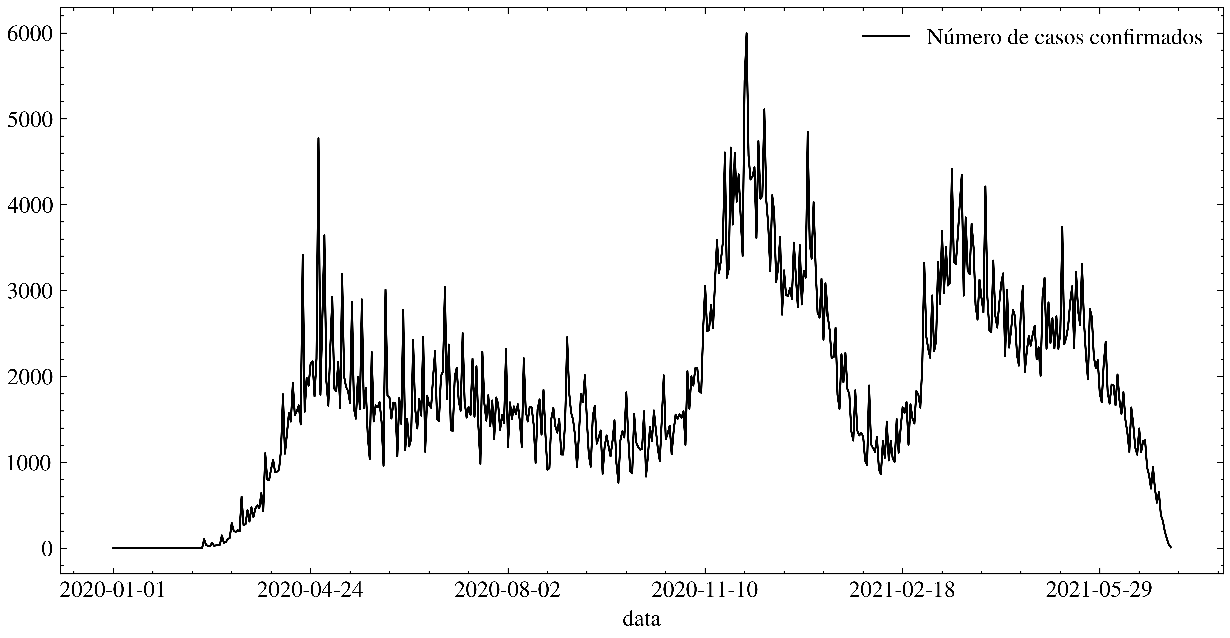
\includegraphics[width=5.0in]{img/casos_confirmados.pdf}
    \caption{Série temporal do número de casos confirmados de COVID-19 no Rio de Janeiro.}\label{fig:casos_confirmados}
\end{figure}

A Figura~\ref{fig:casos_confirmados} mostra que há flutuações a curto pazo, que podem ter sido geradas por diversos fatores na coleta dos dados, como, por exemplo, a subamostragem. Como a coleta dos dados utilizados foi feita de fontes externas e públicas, os experimentos deste se limitaram a trabalhar com o dado como foi disponibilizado, sem aprofundar na avaliação da coleta. Porém, para remover a influência dessas flutuações, foi aplicado o método de médias móveis variando o parâmetro do número de amostras junto à busca de hiperparâmetros para encontrar o melhor ajuste. A Figura~\ref{fig:casos_confirmados_ma} mostra a mesma série temporal com as médias móveis em vermelho considerando-se o parâmetro $n=7$ como exemplo de suavização na flutuação dos valores da série temporal.

\begin{figure}[!htp]
    \centering
    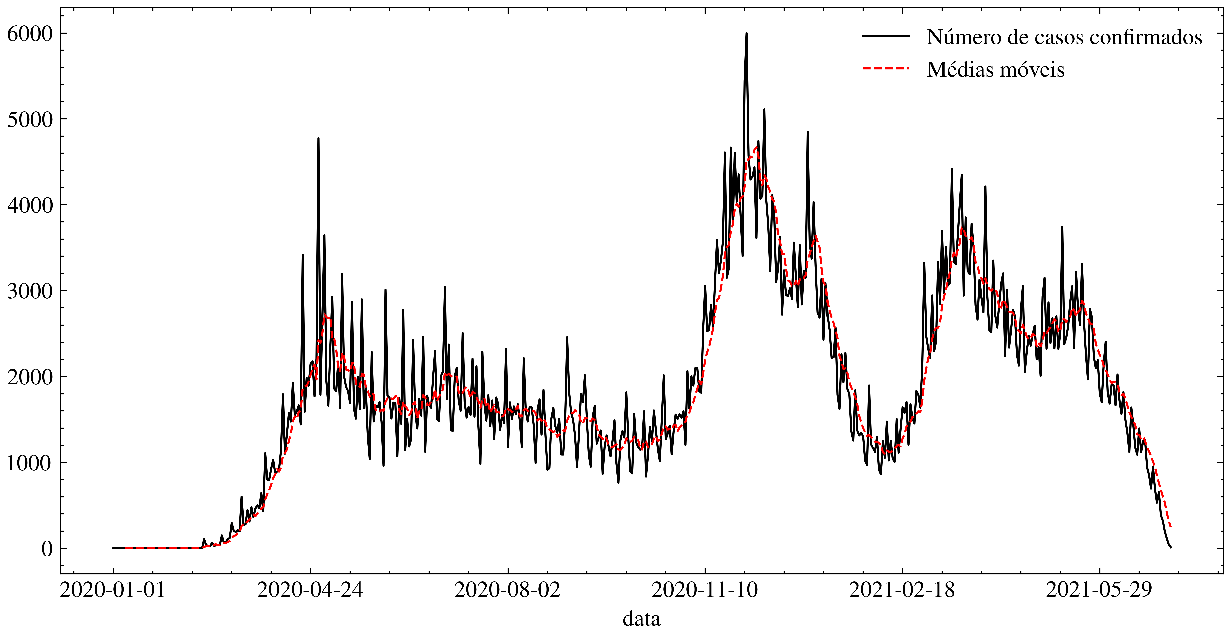
\includegraphics[width=5.0in]{img/casos_confirmados_ma.pdf}
    \caption{Médias móveis do número de casos confirmados de COVID-19 no Rio de Janeiro.}\label{fig:casos_confirmados_ma}
\end{figure}

\FloatBarrier

\subsection{Temperatura mínima diária em Melbourne}
Assim como na conjunto de dados referente ao número de casos confirmados de COVID-19 no Rio de Janeiro~\ref{subsec:casos_confirmados}, os dados de temperatura mínima diária em Melbourne foram baixados através de um \textit{script} Python com o auxílio da biblioteca \textit{requests}. O arquivo pode ser baixado diretamente do GitHub\footnote{$https://raw.githubusercontent.com/jbrownlee/Datasets/master/daily-min-temperatures.csv$} e também pode ser encontrado em um desafio do Kaggle\footnote{$https://www.kaggle.com/paulbrabban/daily-minimum-temperatures-in-melbourne$}.

\begin{figure}[!htp]
    \centering
    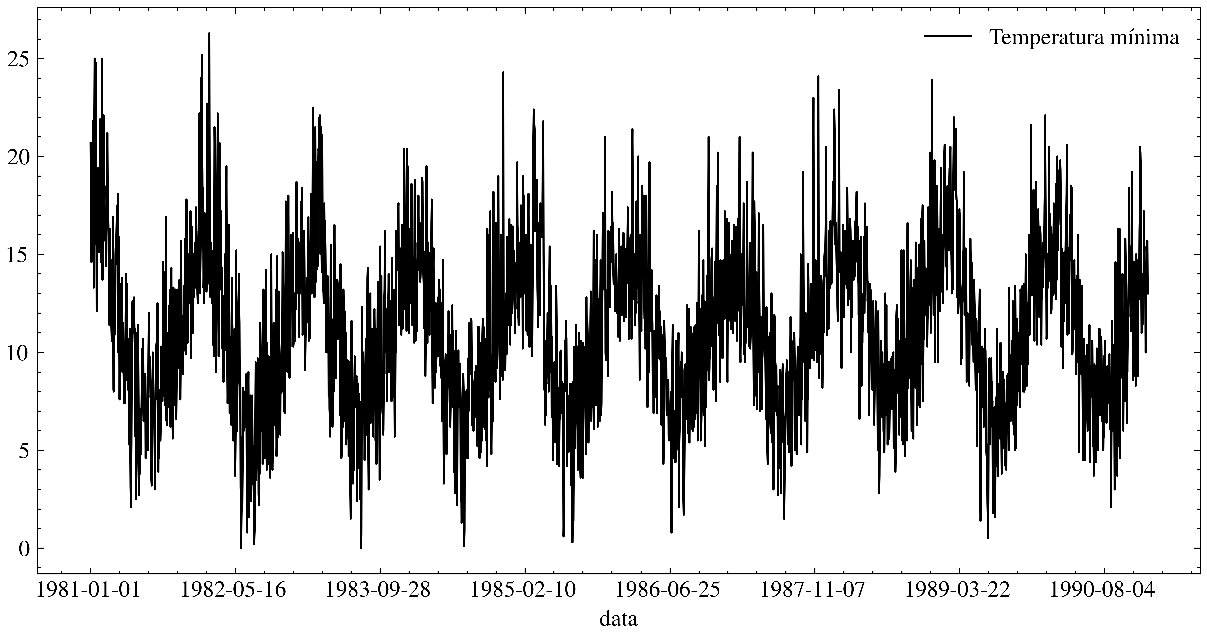
\includegraphics[width=5.0in]{img/temperatura_minima_diaria.pdf}
    \caption{Série temporal da temperatura mínima diária em Melbourne.}\label{fig:temperatura_minima_diaria}
\end{figure}

A Figura~\ref{fig:temperatura_minima_diaria} mostra que a quantidade de observações na série temporal da temperatura mínima diária em Melbourne é muito superior ao número de casos confirmados de COVID-19, e correspondem ao período entre 01/01/1981 e 31/12/1990. Outro ponto divergente é a observabilidade do caráter sazonal com período de um ano. Porém, as flutuações de curto prazo permanecem, e continuam configurando um problema para o ajuste de modelos preditivos que precisam generalizar para realizar inferências mais acertivas.

\begin{figure}[!htp]
    \centering
    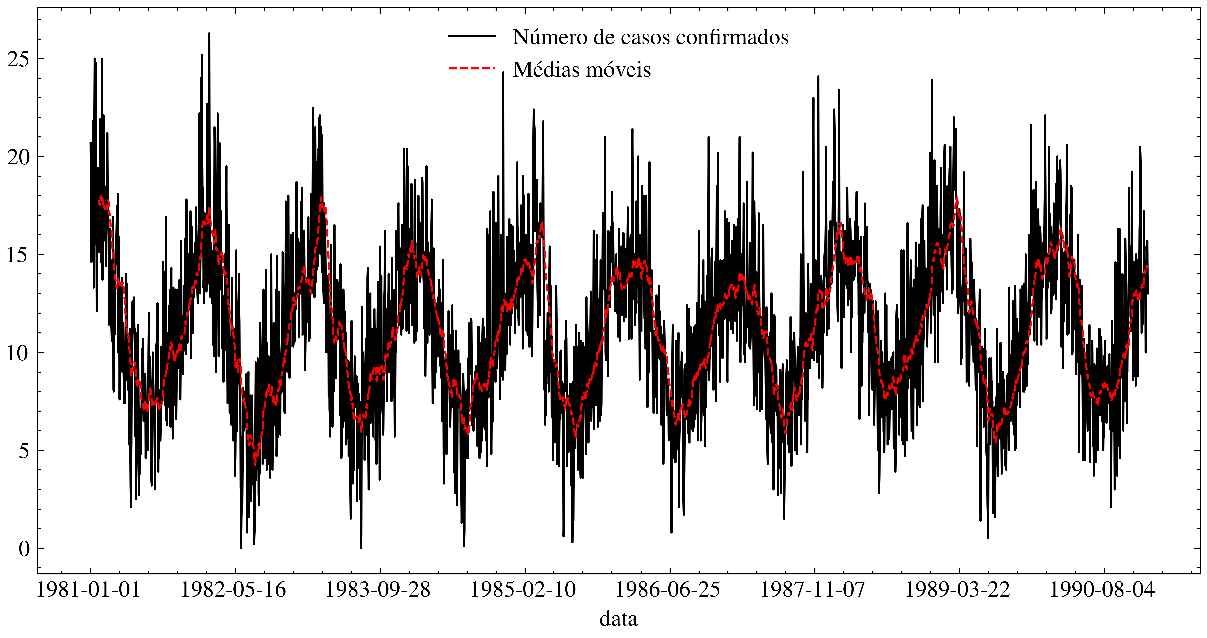
\includegraphics[width=5.0in]{img/temperatura_minima_diaria_ma.pdf}
    \caption{Médias móveis da temperatura mínima diária em Melbourne.}\label{fig:temperatura_minima_diaria_ma}
\end{figure}

A Figura~\ref{fig:temperatura_minima_diaria_ma} mostra as médias móveis da temperatura mínima diária em Melbourne em vermelho. O parâmetro utilizado para gerar esta figura foi $W=30$, que foi escolhido para representação gráfica por se tratar de uma série com aproximadamente um ano de período de sazonalidade.

\FloatBarrier

\subsection{Série temporal sintética}
Uma conjunto de dados foi gerada de forma sintética com o auxílio da biblioteca \textit{numpy} do Python com características criadas artificialmente somando componentes como tendência, sazonalidade, ruído branco e fatores para distorção da estacionaridade seguindo o método apresentado em \citeauthor{syntheticdata}, \citeyear{syntheticdata}\cite{syntheticdata}. Essa série temporal é construída com o objetivo de avaliar a capacidade de generalização dos modelos em cima dos componentes que estes costumam considerar como base, justificando a importância de ter sido gerada sinteticamente.

Em uma série temporal, a tendência é o padrão que evidencia o crescimento ou decrescimento dos valores a longo prazo. Portanto, para compor a série temporal sintética, foi considerada uma função linear crescente como fator de tendência. A Figura~\ref{fig:upward_trend} mostra a componente resultante gerada sinteticamente.

\begin{figure}[!htp]
    \centering
    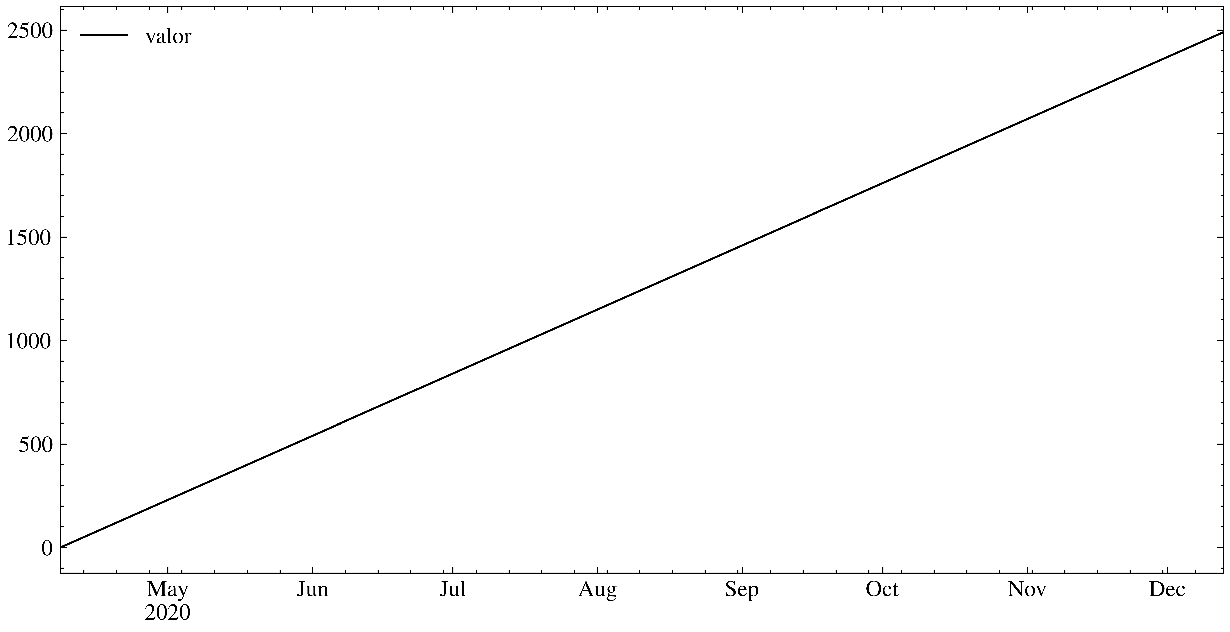
\includegraphics[width=5.0in]{img/upward_trend.pdf}
    \caption{Componente de tendência crescente.}\label{fig:upward_trend}
\end{figure}

A sasonalidade pode ser caracterizada pela presença de variações semelhantes que ocorrem em intervalos regulares de tempo. Então, para simular um comportamento sazonal, foi aplicado um crescimento cúbico seguido de um crescimento quadrático nos primeiros 50 dias, e então esse mesmo padrão foi repetido ao longo de toda a série temporal até o último dado observado. Na Figura~\ref{fig:seasonal_pattern} fica clara a repetição do padrão com as 2 curvas de crescimento seguidas.

\begin{figure}[!htp]
    \centering
    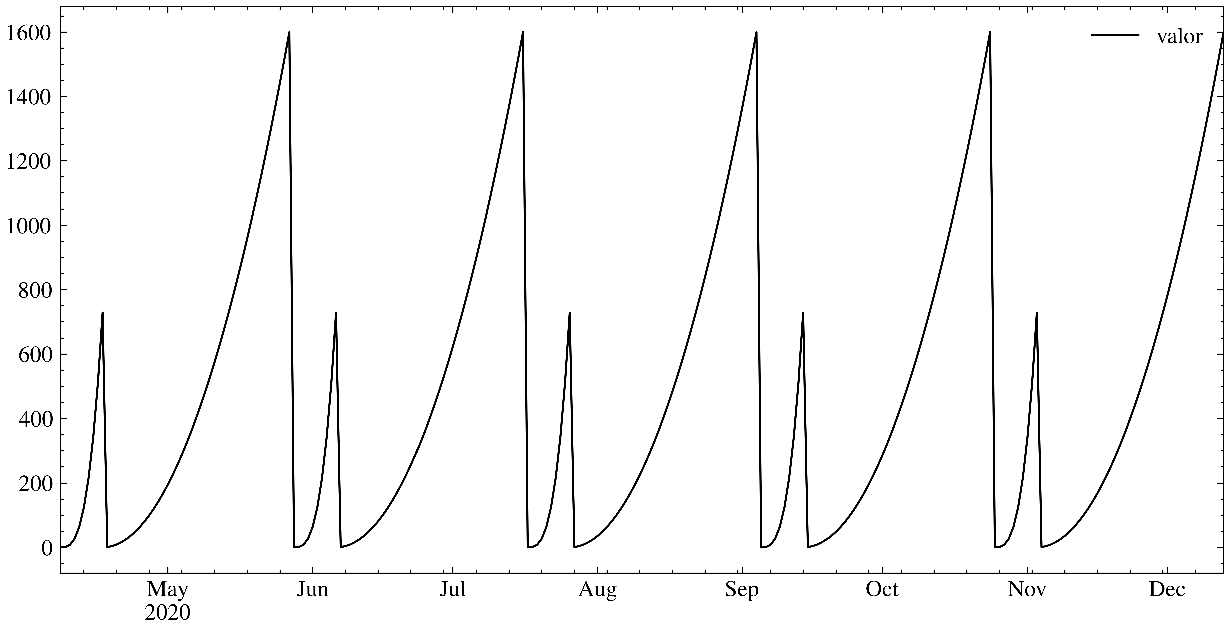
\includegraphics[width=5.0in]{img/seasonal_pattern.pdf}
    \caption{Componente de sazonalidade.}\label{fig:seasonal_pattern}
\end{figure}

O ruído é a parte do sinal que não possui valor semântico, ou seja, são distorções que ocorrem no sinal que podem ter como origem diversos fatores como o equipamento utilizado para fazer a coleta, erro humano, entre outros. Como nenhum sinal na vida real é livre de ruído, para aproximar a série temporal a de um problema real, foi adicionado um sinal de ruído branco gerado de forma pseudo-aleatória conforme apresentado na Figura~\ref{fig:noise}. Além do ruído, também foi adicionado um evento com impacto maior na série temporal com o objetivo de representar um fator inesperado na série. Esse fator pode ser equiparado a qualquer evento que possa alterar de forma disruptiva os dados observados na série temporal. Portanto, como a série possui uma tendência de crescimento, foi gerado um componente decrescente, ilustrado na Figura~\ref{fig:big_event}, nos últimos dias da série para ser somado aos outros componentes e gerar o efeito desejado.

\begin{figure}[!htp]
    \centering
    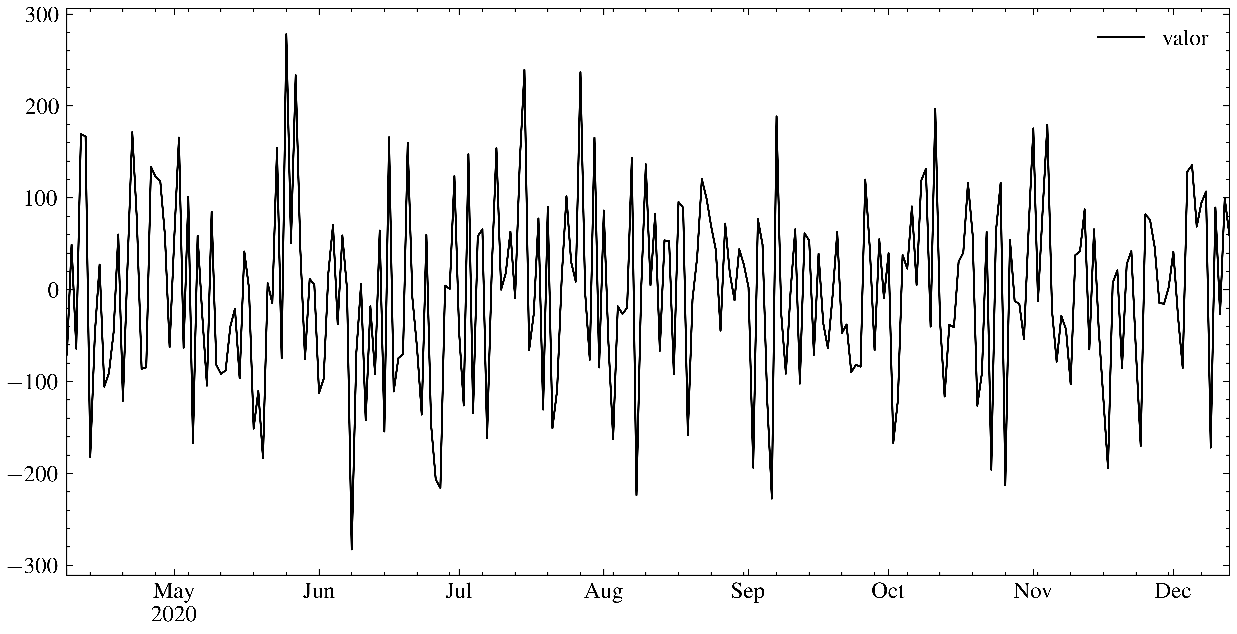
\includegraphics[width=5.0in]{img/noise.pdf}
    \caption{Ruído branco utilizado para compor a série temporal sintética.}\label{fig:noise}
\end{figure}

\begin{figure}[!htp]
    \centering
    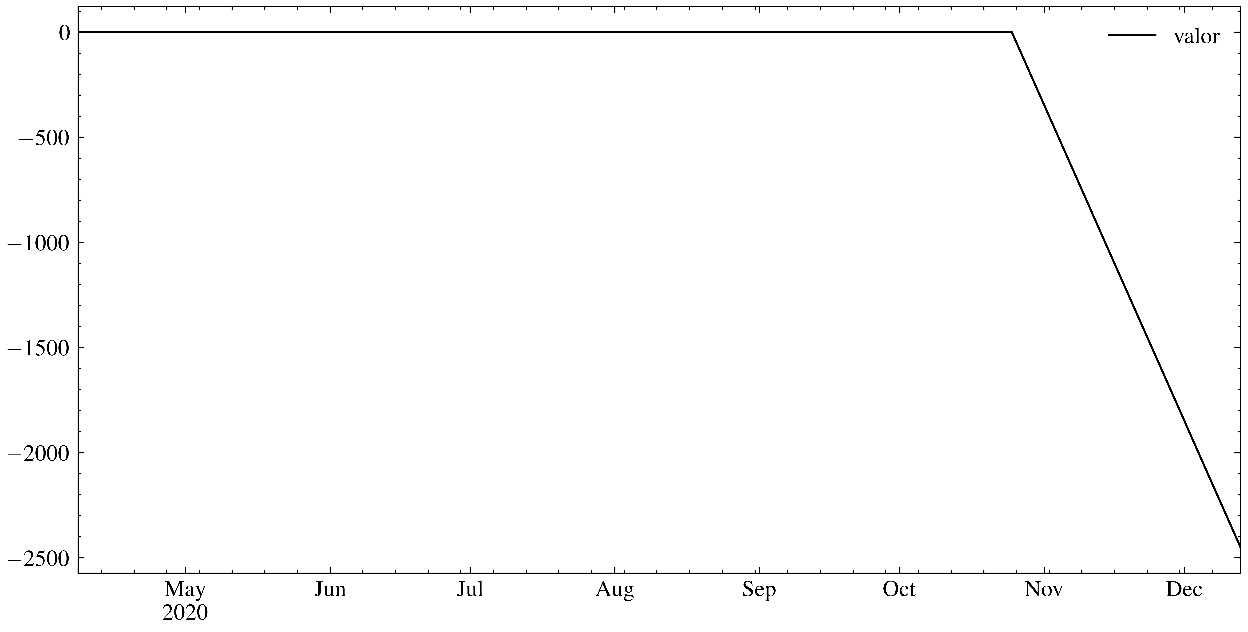
\includegraphics[width=5.0in]{img/big_event.pdf}
    \caption{Componente de evento inesperado descrescente.}\label{fig:big_event}
\end{figure}

Finalmente, após a soma de todos os componentes, é alcançada a série temporal resultante, conforme mostra a Figura~\ref{fig:dados_sinteticos}, onde será possível ajustar os modelos de predição e avaliar a capacidade de generalização de cada um. Como nas séries temporais anteriores, compartilha de flutuações de curto prazo, apesar de menores. Portanto, a Figura~\ref{fig:dados_sinteticos_ma} mostra as médias móveis calculadas com $W=4$ sobre a série temporal sintética. Esse valor foi escolhido na tentativa de suavizar as pequenas flutuações causadas propositalmente pela adição de ruído na composição da série temporal sintética.

\begin{figure}[!htp]
    \centering
    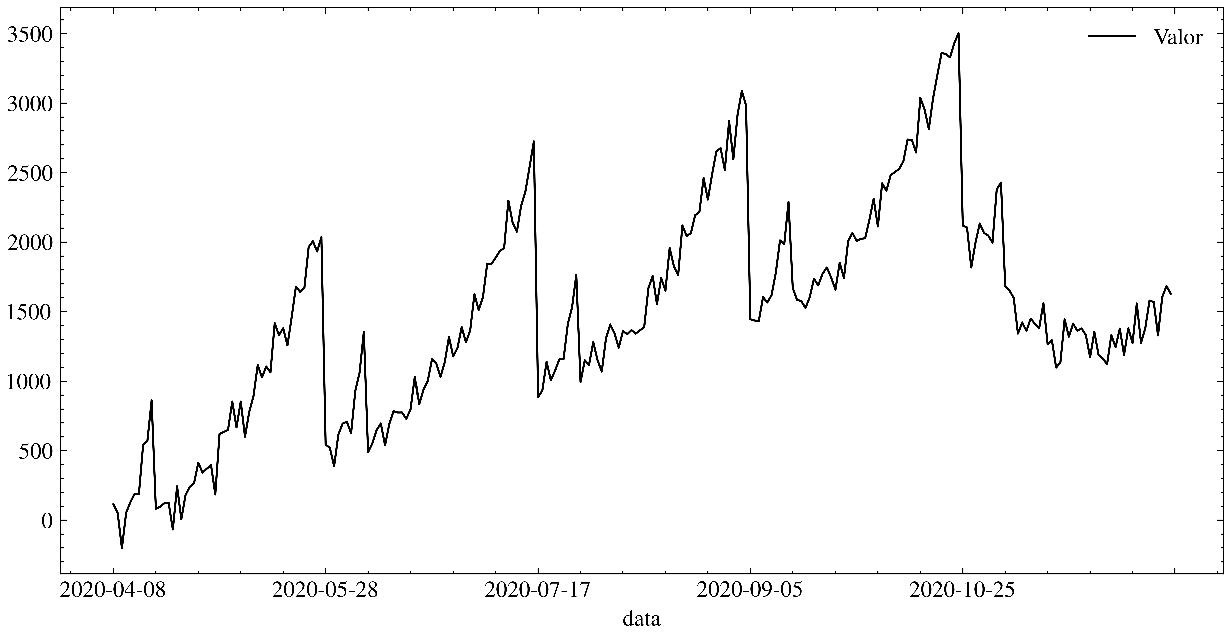
\includegraphics[width=5.0in]{img/dados_sinteticos.pdf}
    \caption{Série temporal gerada sinteticamente.}\label{fig:dados_sinteticos}
\end{figure}


\begin{figure}[!htp]
    \centering
    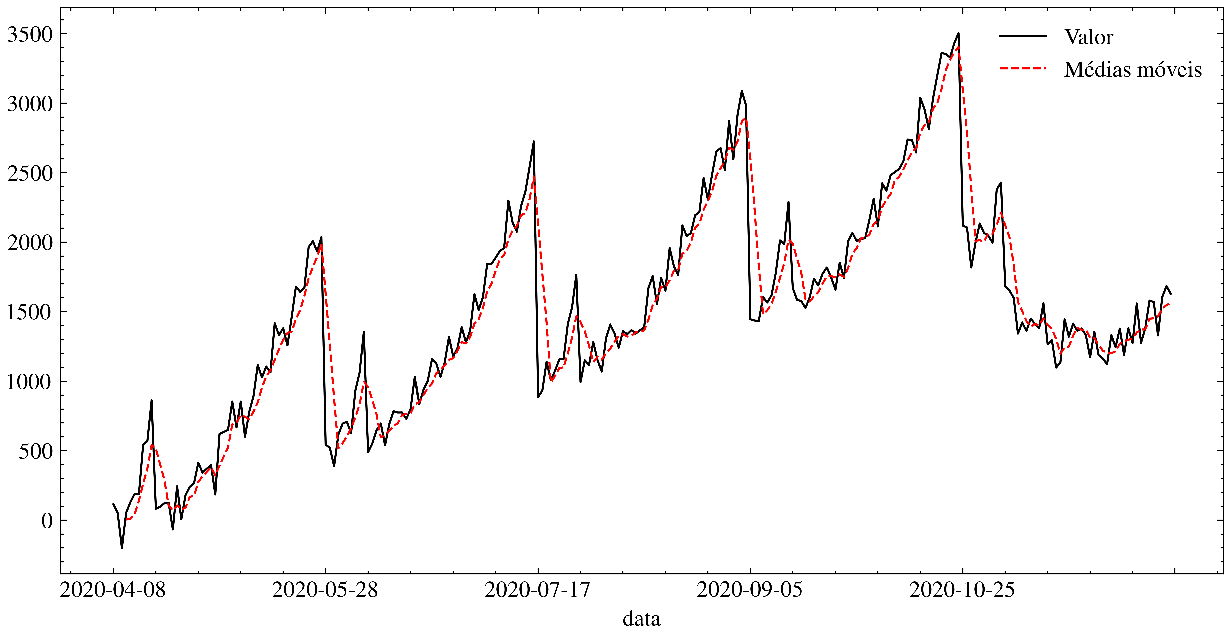
\includegraphics[width=5.0in]{img/dados_sinteticos_ma.pdf}
    \caption{Médias móveis da série temporal gerada sinteticamente.}\label{fig:dados_sinteticos_ma}
\end{figure}

\FloatBarrier

\section{Métricas de avaliação utilizadas}\label{sec:metrics}
Para a avaliação dos modelos preditivos, foram utilizadas quatro métricas de avaliação:  Raiz do Erro Médio Quadrático (\textit{Root Mean Square Error}, RMSE), Erro Médio Absoluto (\textit{Mean Absolute Error}, MAE), Erro Percentual Médio (\textit{Mean Percentage Error}, MPE) e Erro Percentual Absoluto Médio (\textit{Mean Absolute Percentage Error}, MAPE). As métricas foram escolhidas com o objetivo de avaliar o erro de predição dos modelos de diferentes perspectivas. As Equações~\ref{eq:rmse}, \ref{eq:mae}, \ref{eq:mpe} e \ref{eq:mape} consideram $n$ como o número de observações presentes na conjunto de dados, os valores de $y_{i}$ representam o conjunto de valores previstos pelos modelos e $x_{i}$ são os valores observados do conjunto separado para teste.

A Equação~\ref{eq:rmse} descreve o RMSE, que representa a raiz quadrada da média quadrática da diferença entre os valores previstos e observados. O RMSE é uma métrica que pode ser utilizada para comparar diferentes modelos ajustados e avaliados sobre um mesmo conjunto de dados, não sendo indicado para comparações entre conjuntos de dados diferentes. Esse comportamento é justificado pelo fato do RMSE ser uma métrica de acurácia que a escala depende da escala dos dados, como constatado em \cite{HYNDMAN2006679}. O valor de RMSE nunca assume valores negativos, e, em geral, valores menores são melhores que valores maiores. Esta métrica é sensível a erros muito grandes, ou seja, não possui um comportamento estável quando há valores atípicos.

\begin{equation} \label{eq:rmse}
    RMSE=\sqrt{\dfrac{\sum ^{n}_{i=1}\left( y_{i}-x_{i}\right) ^{2}}{n}}
\end{equation}

A métrica expressa pela Equação~\ref{eq:mae}, assim como o RMSE, é uma medida de acurácia. Com isso, compartilha da mesma propriedade de escala. A sua diferença principal, é que seu cálculo é linear, ou seja, as diferenças entre os valores observados e preditos são igualmente ponderadas na média.

\begin{equation} \label{eq:mae}
    MAE=\sum ^{n}_{i=1}\dfrac{\left| y_{i}-x_{i}\right| }{n}
\end{equation}

Diferente das métricas MAE, RMSE e MAPE, a \textit{Mean Percentage Error} (MPE), é uma métrica que considera o sinal do erro, ou seja, erros positivos e negativos se cancelam. Como consequência, a sua fórmula pode ser usada para medir o viés das predições. A Equação~\ref{eq:mpe} mostra como é feito o cáculo da MPE.

\begin{equation} \label{eq:mpe}
    MPE=\dfrac{1}{n}\sum ^{n}_{i=1}\dfrac{x_{i}-y_{i}}{x_{i}}
\end{equation}

A métrica \textit{Mean Absolute Percentage Error} (MAPE), é uma medida de acurácia, assim como a RMSE e MAE. Seu diferencial se dá pelo fato de ter uma interpretabilidade intuitiva comparado às outras métricas. Porém possui alguns defeitos bem conhecidos \cite{CHRISTOFALLIS2015}, como o erro da divisão por 0 e o fato de penalizar mais erros negativos do que erros positivos \cite{MAKRIDAKIS1993527}, levando à escolha de modelos cujo as predições são de valores mais baixos.

\begin{equation} \label{eq:mape}
    MAPE=\dfrac{1}{n}\sum ^{n}_{i=1}\left| \dfrac{y_{i}-x_{i}}{x_{i}}\right|
\end{equation}

\section{Resultados}
Os modelos Prophet, ARIMA e Regression WiSARD tiveram seus hiperparâmetros otimizados através de uma busca exaustiva em grade. Para cada modelo, foi definido um conjunto específico de combinações de hiperparâmetros que formaram um espaço discreto de busca, onde todas as possibilidades foram avaliadas. Os melhores conjuntos de hiperparâmetros encontrados para cada modelo, foram utilizados para uma comparação entre os modelos de acordo com três critérios: erro, tempo de inferência/ajuste e uso de memória RAM para inferência.

\subsection{Avaliação por métricas}\label{subsec:metrics_eval}
Para uma comparação quanto ao erro dos modelos, foram avaliadas as métricas explicadas na Seção~\ref{sec:metrics} para cada configuração possível da grade de hiperparâmetros de cada modelo. Cada modelo teve quatro configurações escolhidas, que foram otimizadas por cada uma das métricas apresentadas. As Tabelas~\ref{tab:covid_results}, \ref{tab:temperature_results} e \ref{tab:synthetic_results} mostram os resultados obtidos para cada conjunto de dados.


\begin{table}[!htp]
    \caption{Tabela de métricas para a conjunto de dados do número de casos confirmados de COVID-19 no Rio de Janeiro.}\label{tab:covid_results}
    \centering
    \begin{tabular}{@{}ccccc@{}} \toprule
        Modelo  & RMSE                & MAPE              & MPE                & MAE                 \\ \midrule
        ARIMA   & \textbf{238.181820} & \textbf{0.254128} & \textbf{-0.060560} & \textbf{194.656193} \\
        ReW     & 261.198655          & 5.029668          & -4.672775          & 226.856128          \\
        Prophet & 1214.961631         & 21.895568         & -21.895568         & 1205.848658         \\ \bottomrule
    \end{tabular}
\end{table}

\begin{table}[!htp]
    \caption{Tabela de métricas para a conjunto de dados da temperatura mínima diária de Melbourne.}\label{tab:temperature_results}
    \centering
    \begin{tabular}{@{}ccccc@{}} \toprule
        Modelo  & RMSE              & MAPE              & MPE                   & MAE               \\ \midrule
        ARIMA   & 1.049886          & 0.060034          & -1.830924e-04         & 0.848392          \\
        ReW     & 0.910288          & \textbf{0.048378} & \textbf{5.457293e-08} & \textbf{0.700003} \\
        Prophet & \textbf{0.905167} & 0.049002          & -1.334196e-04         & 0.707685          \\ \bottomrule
    \end{tabular}
\end{table}

\begin{table}[!htp]
    \caption{Tabela de métricas para a conjunto de dados gerado sinteticamente.}\label{tab:synthetic_results}
    \centering
    \begin{tabular}{@{}ccccc@{}} \toprule
        Modelo  & RMSE                & MAPE              & MPE               & MAE                 \\ \midrule
        ARIMA   & 131.741791          & 0.082449          & 0.006564          & 126.191932          \\
        ReW     & \textbf{126.377103} & \textbf{0.070265} & \textbf{0.000020} & \textbf{101.588470} \\
        Prophet & 169.177431          & 0.100267          & 0.023560          & 153.021037          \\ \bottomrule
    \end{tabular}
\end{table}

Além das tabelas, o Apêndice~\ref{apen:a} mostra a comparação dos modelos para cada métrica através de gráficos de barras.


\subsection{Tempos de execução}
Para medir o tempo de execução, foram utilizados todos os melhores conjuntos de hiperparâmetros encontrados na busca de acordo com cada métrica, ou seja, foram realizados um total de quatro medições para cada modelo para cada conjunto de dados. A medida de tempo do mesmo modelo com diferentes conjuntos de hiperparâmetros pode parecer irrelevante em um primeiro momento, mas pode indicar uma possível sensibilidade de performance dependendo do treinamento. A Tabela~\ref{tab:tempo_ajuste} mostra as medições de tempo feitas no momento da inferência, enquanto a Tabela~\ref{tab:tempo_inferencia} mostra as medições de tempo de inferência dos modelos. As medições de tempo de treinamento foram realizadas em sete rodadas com dez iterações, enquanto as de inferência foram obtidas com sete rodadas de 100 iterações.

\begin{table}[htbp]
    \caption{Tempo de treinamento dos modelos.}\label{tab:tempo_ajuste}
    \centering
    \begin{tabular}{@{}ccccc@{}} \toprule
                                  &                           & \multicolumn{3}{c}{Conjunto de dados}                                                                                       \\ \cmidrule{3-5}
        \multirow{-2}{*}{Modelo}  & \multirow{-2}{*}{Métrica} & \multicolumn{1}{c}{COVID}                      & \multicolumn{1}{c}{Temperatura}               & Sintético                 \\ \midrule
                                  & RMSE                      & \multicolumn{1}{c}{779 ms ± 2.4 ms}            & \multicolumn{1}{c}{3.61 s ± 5.34 ms}          & 38.4 ms ± 383 µs          \\
                                  & MAPE                      & \multicolumn{1}{c}{1.34 s ± 2.11ms}            & \multicolumn{1}{c}{3.61 s ± 4.68 ms}          & 38.3 ms ± 184 µs          \\
                                  & MAE                       & \multicolumn{1}{c}{779 ms ± 1.2 ms}            & \multicolumn{1}{c}{3.61 s ± 8.5 ms}           & 38.4 ms ± 225 µs          \\
        \multirow{-4}{*}{ARIMA}   & MPE                       & \multicolumn{1}{c}{1.61 s ± 1.33 ms}           & \multicolumn{1}{c}{6.36 s ± 9.48 ms}          & 566 ms ± 705 µs           \\ \midrule
                                  & RMSE                      & \multicolumn{1}{c}{\textbf{4.41 ms ± 151 µs}}  & \multicolumn{1}{c}{\textbf{31.2 ms ± 526 µs}} & \textbf{9.97 ms ± 143 µs} \\
                                  & MAPE                      & \multicolumn{1}{c}{\textbf{4.46 ms ± 75.1 µs}} & \multicolumn{1}{c}{\textbf{19.5 ms ± 409 µs}} & \textbf{10.1 ms ± 166 µs} \\
                                  & MAE                       & \multicolumn{1}{c}{\textbf{8.65 ms ± 126 µs}}  & \multicolumn{1}{c}{\textbf{19.3 ms ± 149 µs}} & \textbf{10.5 ms ± 116 µs} \\
        \multirow{-4}{*}{ReW}     & MPE                       & \multicolumn{1}{c}{\textbf{4.41 ms ± 151 µs}}  & \multicolumn{1}{c}{\textbf{64.7 ms ± 549 µs}} & \textbf{8.86 ms ± 123 µs} \\ \midrule
                                  & RMSE                      & \multicolumn{1}{c}{56.5 ms ± 17.9 ms}          & \multicolumn{1}{c}{205 ms ± 176 µs}           & 60.7 ms ± 87 µs           \\
                                  & MAPE                      & \multicolumn{1}{c}{46 ms ± 63.1 µs}            & \multicolumn{1}{c}{179 ms ± 514 µs}           & 60.9 ms ± 174 µs          \\
                                  & MAE                       & \multicolumn{1}{c}{44.6 ms ± 109 µs}           & \multicolumn{1}{c}{180 ms ± 396 µs}           & 61.1 ms ± 177 µs          \\
        \multirow{-4}{*}{Prophet} & MPE                       & \multicolumn{1}{c}{46 ms ± 72.1 µs}            & \multicolumn{1}{c}{203 ms ± 200 µs}           & 68.1 ms ± 178 µs          \\ \bottomrule
    \end{tabular}
\end{table}

\begin{table}[htbp]
    \caption{Tempo de inferência dos modelos.}\label{tab:tempo_inferencia}
    \centering
    \begin{tabular}{@{}ccccc@{}} \toprule
                                  &                           & \multicolumn{3}{c}{Conjunto de dados}                                                                                       \\ \cmidrule{3-5}
        \multirow{-2}{*}{Modelo}  & \multirow{-2}{*}{Métrica} & \multicolumn{1}{c}{COVID}                      & \multicolumn{1}{c}{Temperatura}               & Sintético                 \\ \midrule
                                  & RMSE                      & \multicolumn{1}{c}{960 µs ± 2.51 µs}           & \multicolumn{1}{c}{951 µs ± 14.4 µs}          & 1.92 ms ± 28.5 µs         \\
                                  & MAPE                      & \multicolumn{1}{c}{970 µs ± 1.83 µs}           & \multicolumn{1}{c}{942 µs ± 4.96 µs}          & 1.93 ms ± 33.3 µs         \\
                                  & MAE                       & \multicolumn{1}{c}{958 µs ± 2.81 µs}           & \multicolumn{1}{c}{972 µs ± 8.09 µs}          & 1.92 ms ± 24.8 µs         \\
        \multirow{-4}{*}{ARIMA}   & MPE                       & \multicolumn{1}{c}{959 µs ± 5.72 µs}           & \multicolumn{1}{c}{956 µs ± 7.02 µs}          & 953 µs ± 27.8 µs          \\ \midrule
                                  & RMSE                      & \multicolumn{1}{c}{\textbf{142 µs ± 2.8 µs}}   & \multicolumn{1}{c}{\textbf{149 µs ± 349 ns}}  & \textbf{330 µs ± 4.67 µs} \\
                                  & MAPE                      & \multicolumn{1}{c}{\textbf{87.6 µs ± 1.22 µs}} & \multicolumn{1}{c}{\textbf{106 µs ± 339 ns}}  & \textbf{494 µs ± 12.8 µs} \\
                                  & MAE                       & \multicolumn{1}{c}{\textbf{145 µs ± 2.3 µs}}   & \multicolumn{1}{c}{\textbf{107 µs ± 1.45 µs}} & \textbf{512 µs ± 7.91 µs} \\
        \multirow{-4}{*}{ReW}     & MPE                       & \multicolumn{1}{c}{\textbf{91 µs ± 638 ns}}    & \multicolumn{1}{c}{\textbf{232 µs ± 6.43 µs}} & \textbf{422 µs ± 8.16 µs} \\ \midrule
                                  & RMSE                      & \multicolumn{1}{c}{1.26 s ± 10.7 ms}           & \multicolumn{1}{c}{1.88 s ± 3.79 ms}          & 898 ms ± 768 µs           \\
                                  & MAPE                      & \multicolumn{1}{c}{1.25 s ± 1.59 ms}           & \multicolumn{1}{c}{2.13 s ± 711 µs}           & 906 ms ± 600 µs           \\
                                  & MAE                       & \multicolumn{1}{c}{1.25 s ± 1.29 ms}           & \multicolumn{1}{c}{2.13 s ± 940 µs}           & 898 ms ± 753 µs           \\
        \multirow{-4}{*}{Prophet} & MPE                       & \multicolumn{1}{c}{1.25 s ± 1.26 ms}           & \multicolumn{1}{c}{1.88 s ± 530 µs}           & 899 ms ± 1.24 ms          \\ \bottomrule
    \end{tabular}
\end{table}

\FloatBarrier

\subsection{Uso de memória}
Assim como as medidas de tempo de execução, o uso de memória foi coletado para cada combinação de modelo, conjunto de dados e métrica utilizada para escolha dos hiperparâmetros. Porém, neste caso, a medida de interesse é o uso de memória do modelo ajustado, portanto a Tabela~\ref{tab:memoria} mostra o uso de memória em MiB de cada modelo. As medidas foram realizadas com o auxílio da biblioteca \textit{memory\_profiler}, que possui todas suas especificações documentadas no github\footnote{$https://github.com/pythonprofilers/memory\_profiler\#memory-profiler$}.

\begin{table}[htbp]
    \caption{Uso de memória de cada modelo por métrica otimizada e conjunto de dados.}\label{tab:memoria}
    \centering
    \begin{tabular}{@{}ccccc@{}} \toprule
                                  &                           & \multicolumn{3}{c}{Conjunto de dados}                                                                 \\ \cmidrule{3-5}
        \multirow{-2}{*}{Modelo}  & \multirow{-2}{*}{Métrica} & \multicolumn{1}{c}{COVID}              & \multicolumn{1}{c}{Temperatura}        & Sintético          \\ \midrule
                                  & RMSE                      & \multicolumn{1}{c}{9.086 MiB}          & \multicolumn{1}{c}{43.621 MiB}         & 3.105 MiB          \\
                                  & MAPE                      & \multicolumn{1}{c}{11.383 MiB}         & \multicolumn{1}{c}{43.699 MiB}         & 3.078 MiB          \\
                                  & MAE                       & \multicolumn{1}{c}{8.816 MiB}          & \multicolumn{1}{c}{44.035 MiB}         & 3.359 MiB          \\
        \multirow{-4}{*}{ARIMA}   & MPE                       & \multicolumn{1}{c}{13.734 MiB}         & \multicolumn{1}{c}{50.805 MiB}         & 6.457 MiB          \\ \midrule
                                  & RMSE                      & \multicolumn{1}{c}{\textbf{0.512 MiB}} & \multicolumn{1}{c}{\textbf{1.039 MiB}} & \textbf{0.598 MiB} \\
                                  & MAPE                      & \multicolumn{1}{c}{\textbf{0.000 MiB}} & \multicolumn{1}{c}{\textbf{0.922 MiB}} & \textbf{0.570 MiB} \\
                                  & MAE                       & \multicolumn{1}{c}{\textbf{0.586 MiB}} & \multicolumn{1}{c}{\textbf{0.887 MiB}} & \textbf{0.898 MiB} \\
        \multirow{-4}{*}{ReW}     & MPE                       & \multicolumn{1}{c}{\textbf{0.645 MiB}} & \multicolumn{1}{c}{\textbf{0.809 MiB}} & \textbf{0.562 MiB} \\ \midrule
                                  & RMSE                      & \multicolumn{1}{c}{90.676 MiB}         & \multicolumn{1}{c}{101.699 MiB}        & 89.719 MiB         \\
                                  & MAPE                      & \multicolumn{1}{c}{90.652 MiB}         & \multicolumn{1}{c}{102.074 MiB}        & 89.203 MiB         \\
                                  & MAE                       & \multicolumn{1}{c}{90.621 MiB}         & \multicolumn{1}{c}{102.273 MiB}        & 89.426 MiB         \\
        \multirow{-4}{*}{Prophet} & MPE                       & \multicolumn{1}{c}{90.617 MiB}         & \multicolumn{1}{c}{101.926 MiB}        & 89.277 MiB         \\ \bottomrule
    \end{tabular}
\end{table}

\FloatBarrier

\subsection{Discussão}
Com base nos resultados expostos na Subseção~\ref{subsec:metrics_eval}, é possível concluir que todos os modelos atingiram métricas próximas considerando suas respectivas escalas. Na maioria dos casos, todas as métricas apontaram o mesmo modelo como melhor opção, tendo como exceção apenas a conjunto de dados de temperatura mínima diária em Melbourne, que teve o modelo Prophet apontado como melhor opção ao considerar a métrica RMSE. Ao observar as Tabelas~\ref{tab:temperature_results} e \ref{tab:synthetic_results}, é possível também notar a propriedade das métricas dependentes da escala, conforme descrito na Subseção~\ref{subsec:metrics_eval}. Em geral, a Regression WiSARD obteve a melhor performance para os conjuntos de dados sintética e temperatura mínima diária em Melbourne, enquanto o ARIMA obeteve o melhor resultado para o número de casos confirmados de COVID-19 no Rio de Janeiro. Este último pode ser explicado pela presença da parte integrada do modelo ARIMA, que faz a diferenciação dos dados, permitindo que o modelo fique menos sensível ao fato do conjunto de dados não ser estacionário (característica evidente no conjunto de dados em questão).

Os resultados referentes ao tempo de treinamento, por sua vez, favoreceram o modelo Regression WiSARD, apresentando tempos de treinamento ordens de grandeza menores que o ARIMA e o Prophet. Apesar disto, o Prophet apresentou um tempo de treinamento significativamente menor se comparado ao ARIMA. O tempo de inferência também privilegiou a Regression WiSARD, porém o modelo ARIMA obteve tempos significativamente melhores que o Prophet, se mantendo, em alguns casos, quase na mesma ordem de grandeza dos tempos da Regression WiSARD. O tamanho da conjunto de dados foi uma característica relevante para o tempo de treinamento, dado que houve aumento no tempo medido em conjuntos maiores.

Em relação ao uso de memória RAM, a Regression WiSARD apresentou o menor custo, seguida do ARIMA e do Prophet, respectivamente. Independente da conjunto de dados e do conjunto de hiperparâmetros utilizado, houve unanimidade na comparação de uso de memória entre os três modelos, porém, o ARIMA foi o modelo que mais sofreu variações com o tamanho da conjunto de dados, apesar de sempre se manter com uso de memória inferior ao Prophet.